\documentclass[tikz,border=3pt]{standalone}
% Shared preamble for the v2 figures.
% Fonts: acmart's pdfLaTeX set (Libertine text, newtxmath[libertine]) when
% installed; otherwise Latin Modern. Recompile once Libertine is installed.
\usepackage[T1]{fontenc}
\usepackage{amsmath}
\IfFileExists{libertine.sty}{%
  \IfFileExists{newtxmath.sty}{%
    \usepackage[tt=false,type1=true]{libertine}%
    \usepackage[libertine]{newtxmath}%
  }{\usepackage{lmodern}}%
}{\usepackage{lmodern}}
% Colours: Okabe--Ito-derived, distinguishable in greyscale by luminance
% and always paired with a second cue (line weight, dash, marker shape).
\definecolor{editblue}{HTML}{193E57}  % dark: paths, peeling steps, branch
\definecolor{lawgray}{HTML}{81888C}   % mid grey: constraint sets, context
\definecolor{pointver}{HTML}{D55E00}  % vermillion: forced points, blocks
\newcommand{\lab}[1]{\mathsf{#1}}     % labels in sans serif

\usetikzlibrary{arrows.meta,positioning,calc}


\begin{document}
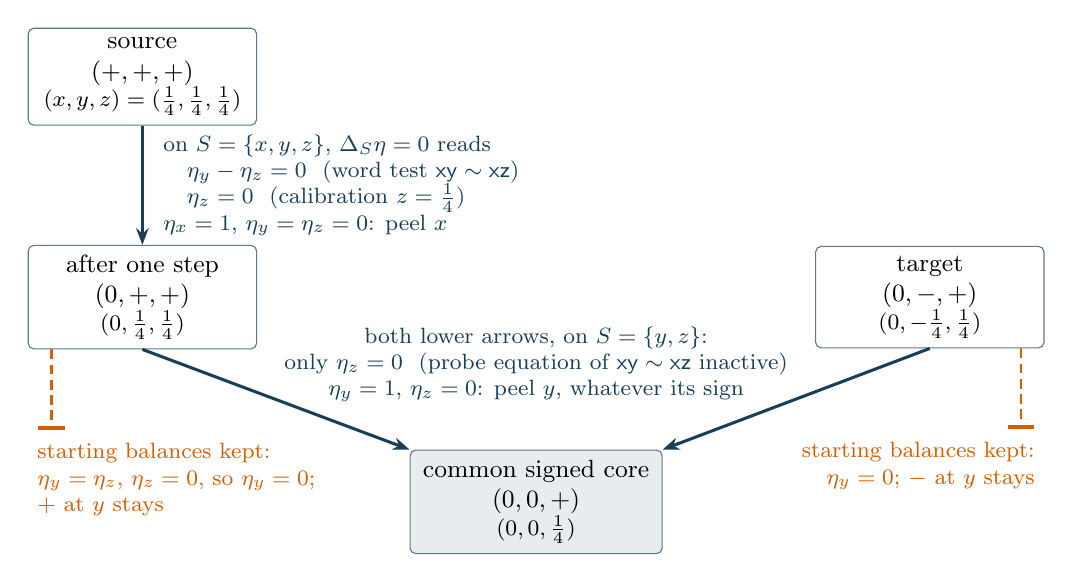
\begin{tikzpicture}[
  every node/.style={font=\small},
  supp/.style={draw=editblue!70, rounded corners=2pt, inner sep=3.5pt,
    minimum width=2.9cm, align=center, fill=white},
  peel/.style={editblue, line width=1.1pt, -{Stealth[length=6pt]}},
  frozen/.style={pointver, line width=0.9pt, dash pattern=on 3.5pt off 2pt},
  eqs/.style={font=\footnotesize, align=left, text=editblue, inner sep=2pt},
]
% rows of nodes by support size |S| = 3, 2, 1
\node[supp] (src) at (0,5.4)
  {source\\$(+,+,+)$\\[-1pt]{\footnotesize$(x,y,z)=(\frac14,\frac14,\frac14)$}};
\node[supp] (mid) at (0,2.6)
  {after one step\\$(0,+,+)$\\[-1pt]{\footnotesize$(0,\frac14,\frac14)$}};
\node[supp] (tgt) at (10.0,2.6)
  {target\\$(0,-,+)$\\[-1pt]{\footnotesize$(0,-\frac14,\frac14)$}};
\node[supp, fill=editblue!10, minimum width=3.2cm] (core) at (5.0,0.0)
  {common signed core\\$(0,0,+)$\\[-1pt]{\footnotesize$(0,0,\frac14)$}};

% recomputed peeling steps, labelled with Delta_S eta = 0 on their support
\draw[peel] (src.south) -- (mid.north)
  node[midway, right=5pt, eqs]
  {on $S=\{x,y,z\}$, $\Delta_S\eta=0$ reads\\
   \quad $\eta_y-\eta_z=0$ \ (word test $\lab{x}\lab{y}\sim\lab{x}\lab{z}$)\\
   \quad $\eta_z=0$ \ (calibration $z=\frac14$)\\
   $\eta_x=1$, $\eta_y=\eta_z=0$: peel $x$};
\draw[peel] (mid.south) -- (core.north west);
\draw[peel] (tgt.south) -- (core.north east);
\node[eqs, align=center] at (5.0,1.75)
  {both lower arrows, on $S=\{y,z\}$:\\
   only $\eta_z=0$ \ (probe equation of $\lab{x}\lab{y}\sim\lab{x}\lab{z}$ inactive)\\
   $\eta_y=1$, $\eta_z=0$: peel $y$, whatever its sign};

% starting support's balance equations kept at {y,z}: y never peels
\draw[frozen] ([xshift=0.3cm]mid.south west) -- ++(0,-1.0) coordinate (fa);
\draw[frozen] ([xshift=-0.3cm]tgt.south east) -- ++(0,-1.0) coordinate (fb);
\foreach \p in {fa,fb}{
  \draw[pointver, line width=1.3pt] ($(\p)+(-0.17,0)$) -- ($(\p)+(0.17,0)$);
}
\node[anchor=north west, font=\footnotesize, text=pointver, align=left]
  at ([xshift=-0.3cm,yshift=-2pt]fa)
  {starting balances kept:\\$\eta_y=\eta_z$, $\eta_z=0$, so $\eta_y=0$;\\$+$ at $y$ stays};
\node[anchor=north east, font=\footnotesize, text=pointver, align=right]
  at ([xshift=0.3cm,yshift=-2pt]fb)
  {starting balances kept:\\$\eta_y=0$; $-$ at $y$ stays};
\end{tikzpicture}
\end{document}
